% Copyright (c) 2021 Eclipse Arrowhead Project
%
% This program and the accompanying materials are made available under the
% terms of the Eclipse Public License 2.0 which is available at
% http://www.eclipse.org/legal/epl-2.0.
%
% SPDX-License-Identifier: EPL-2.0

The \GlossaryHyperRef{framework-arrowhead}{Arrowhead framework} can be divided into a \GlossaryHyperRef{framework-idea}{framework of ideas} and a \GlossaryHyperRef{framework-software}{framework of software}, as shown in Figure \ref{fig:framework}.
The former division concerns the assumptions, concepts, values and practices that frame the problem domain of \textit{coordinating dynamic \GlossaryHyperRef{system-automation}{automation systems}}.
The latter division concerns the software \GlossaryHyperRef{specification-software}{specifications} and \GlossaryHyperRef{implementation-software}{implementations} meant to address that problem domain.
In this section, we provide an overview of the primary \textit{concepts} of the Arrowhead framework.
While \textit{assumptions} and \textit{values} may be possible derive from this overview, no other framework aspects are considered here or in the rest of this document.

\vfill

\begin{figure}[ht!]
  \centering
  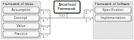
\includegraphics[scale=0.9]{figures/framework}
  \caption{
    The two subframeworks of the Arrowhead framework, concerned with ideas and software.
  }
  \label{fig:framework}
\end{figure}

\vspace*{-3mm}

\subsection{Stakeholders and Artifacts}

There are two kinds of members of the world of Arrowhead, (1) \GlossaryHyperRef{stakeholder}{stakeholders} and (2) \GlossaryHyperRef{artifact}{artifacts}, as depicted in Figure \ref{fig:world}.
The former denotes a \GlossaryHyperRef{person}{person} or \GlossaryHyperRef{organization}{organization} engaged in an Arrowhead enterprise, while the latter is any thing or object, tangible or intangible, that could be relevant to consider as part of such an enterprise.
Stakeholders \GlossaryHyperRef{owner}{own}, \GlossaryHyperRef{supplier}{supply}, \GlossaryHyperRef{developer}{develop}, \GlossaryHyperRef{operator}{operate}, and \GlossaryHyperRef{user}{use} artifacts, among many other possible activities.
It is their business needs and ambitions that govern what and how Arrowhead artifacts are employed.

\vfill

\begin{figure}[ht!]
  \centering
  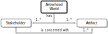
\includegraphics[scale=0.9]{figures/world}
  \caption{
    The two kinds of members of the Arrowhead world: stakeholders and artifacts.
  }
  \label{fig:world}
\end{figure}

\vspace*{-3mm}

\subsection{Devices, Systems and Services}

The most essential types of artifacts in the world of Arrowhead are (1) \GlossaryHyperRef{device}{hardware devices}, (2) \GlossaryHyperRef{system}{software systems} and (3) \GlossaryHyperRef{service}{services}, all shown in Figure \ref{fig:device-system-service}.
\textit{Hardware devices}, or just \textit{devices}, are physical machines, such as servers, robots or tools, able to maintain, or \GlossaryHyperRef{hosting-system}{\textit{host}}, \textit{software systems}.
A software system, or just \textit{system}, is a \GlossaryHyperRef{communication}{communicating} \GlossaryHyperRef{instance-software}{software instance} that \GlossaryHyperRef{provision-service}{provides} \textit{services}.
Every service represents a set of tasks a system can perform for other systems.
Those tasks are concretely represented by a set of \GlossaryHyperRef{operation-service}{operations} that system can execute as requested by other systems.
A service may be concerned with manufacturing, repairs, analysis, or any other physical or virtual activity.
Each of its operations is dedicated to one aspect of its concern.
A service providing control over a door could, for example, have one operation for checking if the door is open and another for opening and closing it.
Service operations can be executed, or \GlossaryHyperRef{consumption-service}{\textit{consumed}}, by other systems or \GlossaryHyperRef{person}{persons}.

\vfill

\begin{figure}[ht!]
  \centering
  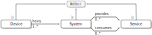
\includegraphics[scale=0.9]{figures/device-system-service}
  \caption{
    Hardware devices \textit{host} software systems, which \textit{provide} services.
    Each of these is an artifact.
  }
  \label{fig:device-system-service}
\end{figure}

\vspace*{-3mm}

\subsection{Service Provision and Consumption}

\GlossaryHyperRef{communication}{Communication} between systems is formulated in terms of the \GlossaryHyperRef{provision-service}{provision} and \GlossaryHyperRef{consumption-service}{consumption} of \GlossaryHyperRef{service}{services}.
\GlossaryHyperRef{system}{Systems} may \textit{provide} services, which other systems can \textit{consume} by sending \GlossaryHyperRef{message}{messages}, as depicted in Figure \ref{fig:service-consumption}.

\begin{figure}[ht!]
  \centering
  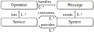
\includegraphics[scale=0.9]{figures/service-consumption}
  \caption{
    Systems consume services by sending messages to the providers of those services.
    Those providers then pass on the messages they receive to their service operations, which interpret and handle them.
  }
  \label{fig:service-consumption}
\end{figure}

When a providing system receives a message from a consuming system, it passes it on to the \GlossaryHyperRef{operation-service}{service operation} specified in that message, as described in Sections \ref{sec:concepts:service} and \ref{sec:concepts:interface}.
The operation receiving the message will then handle it by performing whatever action it describes, given that the message is \GlossaryHyperRef{message-valid}{valid} and \GlossaryHyperRef{message-permitted}{permitted}.
This handling may entail sending additional messages to other systems, starting or stopping various kinds of automation routines, reading from sensors, electronically signing contracts, sending notifications to an \GlossaryHyperRef{operator}{operator}, among many other possible examples.

\subsection{System Composition}

When certain \GlossaryHyperRef{system}{systems} \GlossaryHyperRef{consumer-service}{consume} each other's \GlossaryHyperRef{service}{services}, they form a \GlossaryHyperRef{system-of-systems}{system-of-systems}.
Such a system-of-systems is able to perform activities none of its constituent \GlossaryHyperRef{subsystem}{subsystems} could perform on its own.
Two kinds of system-of-systems have particular significance in the context of the \GlossaryHyperRef{framework-arrowhead}{Arrowhead framework}.
These are (1) the \GlossaryHyperRef{cloud-local}{local cloud}, and (2) the \GlossaryHyperRef{system-of-local-clouds}{system-of-local-clouds}, both depicted in Figure \ref{fig:system-of-systems}.

\begin{figure}[ht!]
  \centering
  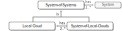
\includegraphics[scale=0.9]{figures/system-of-systems}
  \caption{
    The two primary kinds of Arrowhead systems-of-systems: the local cloud and the system-of-local-clouds.
  }
  \label{fig:system-of-systems}
\end{figure}

A \textit{local cloud} is a set of systems engaged in some form of physical activity that makes those systems physically bound to a particular location.
Local clouds come in many shapes and forms.
They may be completely stationary, completely mobile, or consist of both stationary and mobile devices.
Smelting stations, drone command centers, assembly lines, power distribution centers and satellite systems are a few examples of possible local clouds.

A \textit{system-of-local-clouds} is a set of cooperating local clouds, each kept distinct from the other local clouds by some form of \GlossaryHyperRef{boundary-cloud}{boundary}.
Boundaries may be organizational, physical, security-related, and so on.
Every system-of-local-clouds contains at least one local cloud that depends on another local cloud to perform some activity of relevance.
A systems-of-local-clouds could be formed by a set of weather stations, the robots of some collaborating parties at a mining site, the various departments of a manufacturing plant, the carriers of a supply chain, and so on.
